\documentclass[apj]{emulateapj}
%\documentclass[12pt,preprint]{aastex}

\newcommand{\kms}{km~s$^{-1}$}
\newcommand{\mgii}{\textrm{Mg}~\textsc{ii}}
\newcommand{\nev}{[\textrm{Ne}~\textsc{v}]}
\newcommand{\oii}{[\textrm{O}~\textsc{ii}]}
\newcommand{\oiii}{[\textrm{O}~\textsc{iii}]}
\newcommand{\msun}{M$_{\odot}$}
\newcommand{\mstar}{M$_{*}$}
\newcommand{\units}{M$_{\odot}$~yr$^{-1}$~kpc$^{-2}$}
\newcommand{\lrest}{\lambda_{\textnormal{\scriptsize{rest}}}}
\newcommand{\lobs}{\lambda_{\textnormal{\scriptsize{obs}}}}
\newcommand{\sigmasfr}{\Sigma_{\textnormal{\scriptsize{SFR}}}}
\newcommand{\sfrir}{\textnormal{SFR}_{\textnormal{\scriptsize{IR}}}}
\newcommand {\apgt} {\ {\raise-.5ex\hbox{$\buildrel>\over\sim$}}\ }
\newcommand {\aplt} {\ {\raise-.5ex\hbox{$\buildrel<\over\sim$}}\ }

\shorttitle{Compact Starbursts Revealed by HST and WISE}
\shortauthors{Diamond-Stanic et al.}

\begin{document}

%\title{HST and WISE Reveal Compact Starbursts Driving 1000
%  \kms\ Outflows}

\title{In the Crucible: Massive Compact Galaxies with High-Velocity
  Outflows and Eddington-Limited Star Formation}

\author{Aleksandar M. Diamond-Stanic\altaffilmark{1,2}, John
  Moustakas\altaffilmark{1}, Christy A. Tremonti\altaffilmark{3},
  Alison L. Coil\altaffilmark{1}, Ryan C. Hickox\altaffilmark{4}, Aday
  Robaina\altaffilmark{5}, Gregory H. Rudnick\altaffilmark{6}, \& Paul
  Sell\altaffilmark{3} }

\altaffiltext{1}{Center for Astrophysics and Space Sciences,
  University of California, San Diego, La Jolla, CA 92093, USA}
\altaffiltext{2}{Center for Galaxy Evolution Fellow}
\altaffiltext{3}{Department of Astronomy, University of
  Wisconsin-Madison, Madison, WI 53706, USA}
\altaffiltext{4}{Department of Physics and Astronomy, Dartmouth
  College, Hanover, NH 03755, USA} 

\altaffiltext{5}{Institut de Ci{\'e}ncies del Cosmos, University of
  Barcelona, 08028 Barcelona, Spain}

\altaffiltext{6}{Department of Physics and Astronomy, University of
  Kansas, Lawrence, KS 66045, USA}

\begin{abstract}

We present the discovery of compact, obscured star formation in
galaxies that exhibit $\gtrsim1000$~\kms\ outflows.  Using optical
morphologies from the Hubble Space Telescope and infrared photometry
from the Wide-field Infrared Survey Explorer, we estimate star
formation rate (SFR) surface densities that approach
$\sigmasfr\approx5000$~\msun~yr$^{-1}$~kpc$^{-2}$.  This is comparable
to the Eddington limit from radiation pressure on dust grains.  We
argue that feedback associated with a compact starburst in the form of
radiation pressure from massive stars and ram pressure from supernovae
and stellar winds is sufficient to launch the high-velocity outflows
we observe, without the need to invoke feedback from an active
galactic nucleus.

\end{abstract}

\keywords{galaxies: evolution --- galaxies: kinematics and dynamics
  --- galaxies: ISM --- galaxies: starburst}

\section{Introduction}

The central regions of elliptical galaxies are thought to form in
compact starbursts \citep[e.g.,][]{kor09,hop09}.  Feedback associated
with such starbursts can produce outflows driven by thermal energy
from supernova explosions \citep[e.g.,][]{che85}, stellar winds
\citep[e.g.,][]{lei92}, and momentum input from both supernova ram
pressure and radiation pressure on dust grains \citep[e.g.,][]{mur05}.
It has been argued that such feedback imposes a limit on the maximum
star-formation rate surface density ($\sigmasfr$) for starbursts
\citep[e.g.,][]{leh96,meu97,mur05,tho05} and the maximum stellar
surface density for elliptical galaxies and star clusters
\citep[e.g.,][]{hop10}.

% The relative importance of momentum injection versus thermal heating
% may vary as a function of galaxy mass \citep[e.g.,][]{hop12}, with
% thermal heating being less efficient in galaxies with larger gas
% densities and shorter cooling times.  Massive star clusters with large
% gas surface densities are a potential launching point for
% galactic-scale outflows driven by radiation pressure
% \citep[e.g.,][]{mur11}.

Galactic winds are ubiquitous in star-forming galaxies at all
redshifts and generally exhibit outflow velocities in the
100--500~\kms\ range
\citep[e.g.,][]{hec00,sha03,mar05,rup05,wei09,rub10,ste10}.  Thus, the
discovery of $|v|>1000$~\kms\ outflows in a sample of massive
($\textnormal{\mstar}\approx10^{11}$~\msun) post-starburst galaxies at
$z\sim0.6$ by \citet{tre07} suggested that a more energetic source,
such as feedback from an accreting supermassive black hole
\citep[e.g.,][]{sil98,dim05,deb12}, could have been responsible for
launching the winds \citep[see][for a recent review]{fab12}.

However, it also plausible that feedback from a compact starburst
could expel gas with such large velocities.  Indeed, there is evidence
for a positive correlation between outflow velocity and starburst
luminosity \citep[e.g.,][]{mar05,rup05,tre07}, albeit with significant
scatter.  Furthermore, \citet{hec11} recently found outflows with
maximum velocities reaching $-1500$~\kms\ in a sample of local
starbursts with compact nuclei, and argued that such velocities could
be explained by feedback from massive stars.

% $|v|\gtrsim1000$~\kms\

In this Letter, we present results for a sample of massive galaxies at
$z\sim0.6$ that exhibit $|v|\apgt1000$~\kms\ outflows, expanding on
the sample from \citet{tre07}.  We seek to test whether the energetic
outflows in these galaxies could have been driven by feedback from
starbursts with very large star-formation rate (SFR) surface densities
($\sigmasfr$).  Our analysis combines galaxy sizes obtained with the
Hubble Space Telescope (HST) with star-formation rates and stellar
masses estimated from WISE, Spitzer, SDSS, and GALEX photometry.

% For example, there is evidence for a positive correlation between
% outflow velocity and starburst luminosity \citep[e.g.,][]{mar05},
% albeit with significant scatter.  Furthermore, \citet{hec11} recently
% found outflows reaching velocities of $-1500$~\kms\ in a sample of
% local starbursts with compact nuclei, and argued their higher
% velocities could be explained by feedback exerted by a large number of
% massive stars that are confined to a small radius.

% [which has been invoked theoretically as
%  a mechanism to quench star formation in galaxies,

% Winds are also common in active galactic nuclei (AGNs) with velocities
% in the 1000--20,000~\kms range \citep[e.g., ][]{cre03}, although it is
% unclear whether AGN feedback plays an important role in regulating
% star formation in galaxies.  There is clear observational evidence
% that active galactic nuclei (AGNs) produce outflows
% \citep[e.g.,][]{cre03} and that the outflowing gas can extend to
% $>$kpc scales \citep[e.g.,][]{rup11}, it is unclear whether such
% feedback plays an important role globally in quenching star formation.

% Feedback from massive stars and active black holes has important
% implications for galaxy evolution (e.g., luminosity function, star
% formation, galaxy color bi-modality, mass-metallicity relation,
% enrichment of IGM).  



% Feedback from accreting supermassive black holes has also been invoked
% theoretically as a mechanism for quenching star formation in galaxies
% \citep[e.g.,][]{sil98,gra04,dim05}.  There is clear observational
% evidence that active galactic nuclei (AGNs) produce outflows
% \citep[e.g.,][]{cre03} and that the outflowing gas can extend to
% $>$kpc scales \citep[e.g.,][]{rup11}, but it is unclear whether such
% feedback plays an important role globally in quenching star formation
% and shaping the galaxy mass function.



% and optical spectra ($\lrest=2500$-5200~\AA)

%  The spectral region surrounding the
%  \mgii~$\lambda\lambda2796,2803$ absorption alines, which are used to
%  measure outflow velocities, is highlighted in both wavelength and
%  velocity space.

%  and are scaled to match the WISE channel 2 photometry ($\lobs=4.6$~$\mu$m)
% (\mgii~$\lambda2796$ is plotted in blue and \mgii~$\lambda2803$ is plotted in red)



\section{Analysis}

%\subsection{HST/WFC3 Imaging}
\subsection{Morphologies and Sizes}

Our sample derives from 29 galaxies targeted for HST/WFC3 imaging in
programs 12019 and 12272 (PI: C. Tremonti).  Using the F814W filter on
the UVIS channel, which has $0.04\arcsec$ pixels and
$\textnormal{FWHM}=0.074\arcsec$, we obtained $4\times10$~min
exposures in a single orbit for each galaxy.  The dithered images were
processed with
MultiDrizzle\footnote{http://stsdas.stsci.edu/multidrizzle/} to
produce science mosaics with $0.02\arcsec$ pixels.  For each galaxy,
we use GALFIT \citep{pen02,pen10} to model the two-dimensional surface
brightness profile with a single Sersic component, using stars in the
images to construct the model point-spread function (PSF).  The Sersic
index (n) and effective radius ($r_e$) are free parameters in the
model.  In cases where the best-fit model returns $n>4$, we also fit
an $n=4$ de Vaucouleurs model \citep{dev48}, yielding a larger $r_e$
value (due to the covariance between $n$ and $r_e$), and we use these
these larger effective radii in our analysis.

For this paper, we are most interested in the galaxies with the
largest $\sigmasfr$ values, which also have the smallest effective
radii.  We show the HST images for three high-$\sigmasfr$ galaxies in
Figure~\ref{fig:seds}.  In all three cases, the single-component model
GALFIT accounts for $>85\%$ of the total flux.  The residuals show
diffuse emission that is consistent with these systems being
late-stage galaxy mergers after final coalescence, although we defer a
detailed comparison of the observed morphologies with expectations
from merger simulations to future work.

For the most compact galaxy (J0905+5759, $r_e=0.013\arcsec$ or
100~pc), we also show the observed one-dimensional surface brightness
profile in the bottom-right panel of Figure~\ref{fig:profile}.  We
compare to the profiles of six stars in the same image, the best-fit
de Vaucouleurs model, and a de Vaucouleurs model with a larger
effective radius ($r_e=0.04\arcsec$, the native WFC3/UVIS pixel size,
which corresponds to a physical scale of 290~pc).  This comparison
illustrates that this galaxy, while only marginally resolved with an
effective radius that is $\sim20\%$ of the image FWHM, is clearly more
extended than a point source.

For such a compact source, there is significant uncertainty in our
$r_e$ measurement given uncertainties in the model PSF.  To quantify
this uncertainty, we used TinyTim to generate a model PSF that is
artificially narrower than the stars in the image (convolving the
output of tiny2 with a $\textnormal{FWHM}=0.04\arcsec$ Gaussian,
whereas the image FWHM is $0.074\arcsec$) and found that this
increased the effective radius in the GALFIT model by a factor of two.
We also fit a two-component PSF+Sersic model, but found that the
Sersic component dominates the fit, yielding a similar effective
radius.  Furthermore, the spectrum of the galaxy shows no evidence for
an AGN contribution to the $I$-band continuum (see
Figure~\ref{fig:spectra}), so there is no clear motivation for
including an unresolved, point-source component in the model.  We
conclude that this galaxy is quite compact and that our $r_e$ estimate
of 100~pc, while uncertain, is likely accurate within a factor of two.

\begin{figure}[!t]
%\includegraphics[angle=90,scale=0.68]{sigmasfr_datafigure.ps}
\includegraphics[angle=0,scale=0.41]{3seds.ps}
\caption{Left: Observed UV--IR SEDs ($\lrest=0.1$--15~$\mu$m) for
  three galaxies with large SFR surface densities
  ($\sigmasfr>3000$~\units).  We show stellar population fits to the
  $\lrest=0.1$--3~$\mu$m emission (black solid line) and three
  templates for dust emission \citep[M82 starburst, Arp 220 starburst,
    and obscured quasar;][]{pol07}.  The starburst templates provide
  reasonable fits to the $\lobs=12$ and 22~$\mu$m WISE photometry,
  while the quasar template does not.  Right: HST/WFC3 F814W images
  (probing $\lrest\approx5000$~\AA) showing that these galaxies are
  dominated by a compact nucleus.}
\label{fig:seds}
\end{figure}
% scaled to the WISE $\lobs=4.6~\mu$m flux.

\begin{figure}[!t]
\includegraphics[angle=0,scale=0.41]{profile.ps}
\label{fig:profile}
\caption{One-dimensional surface brightness profile for J0905+5759,
  which has the smallest effective radius in the sample.  The observed
  profile is shown as the solid black line, and the profiles of six
  stars in the same image are shown in blue.  The best-fit de
  Vaucouleurs profile with $r_e=100$~pc is shown as a dashed red line,
  and for comparison a broader profile with $r_e=0.04\arcsec=290$~pc
  is shown as the dotted green line.  This galaxy is quite compact,
  but is more extended than a point source.}
\end{figure}



%\subsection{Photometry, Star Formation Rates, and Stellar Masses}
\subsection{Star Formation Rates and Stellar Masses}

We gathered photometry from the All-Sky Release of the Wide-field
Infrared Survey Explorer \citep[WISE,][]{wri10}, the Seventh Data
Release of the Sloan Digital Sky Survey \citep[SDSS,][]{aba09}, and
General Release 6 from the Galaxy Evolution Explorer
\citep[GALEX,][]{mar05galex}.  We also obtained $5\times30$~sec
dithered exposures at 3.6~$\mu$m and 4.5~$\mu$m for all sources with
the Infrared Array Camera \citep{faz04} on the Spitzer Space Telescope
\citep{wer04} as part of General Observer program 60145 (PI:
C. Tremonti).  We used the post--basic calibrated data to perform
aperture photometry on all sources, and we also used the
APEX\footnote{http://irsa.ipac.caltech.edu/data/SPITZER/docs/dataanalysistools/tools/mopex/}
point-source extraction software for photometry of sources in crowded
fields.  All the photometry was corrected for Galactic extinction
based on the \citet{sch98} dust maps.  We show spectral energy
distributions (SEDs) for the three high-$\sigmasfr$ galaxies in
Figure~\ref{fig:seds}.

We estimate IR-based star-formation rates for the 25/29 galaxies with
WISE 12 or 22~$\mu$m detections by fitting \citet{cha01} templates to
their 12 and 22~$\mu$m fluxes.  For the 14/29 galaxies with 22~$\mu$m
detections, this yields SFRs that agree with those obtained from the
\citet{ruj12} method based on 24~$\mu$m luminosity with a scatter of
0.05~dex.  We note that several authors have shown that the shape of
the IR SED for star-forming galaxies depends on the surface density of
star formation \citep[e.g.,][]{ruj11,elb11}, with more compact
starbursts having larger total-IR (8--1000~$\mu$m) to mid-IR
(8--24~$\mu$m) ratios.  The extreme $\sigmasfr$ values of our sample
imply large total-IR to mid-IR ratios, characteristic of the most
luminous galaxies in the local universe
\citep[e.g.,][]{cha01,dal02,rie09}.  If we used the most luminous
local templates for the 8/29 sources with SFRs in the ULIRG regime
($\sfrir>200$~\msun~yr$^{-1}$), we would obtain SFRs that are larger
by 0.5~dex than the values we adopt for this paper.

We also estimate star-formation rates and stellar masses based on
stellar population fits to the $\lrest=0.1$--3~$\mu$m SEDs using the
method of \citet{mou11}.  For galaxies with
$\sfrir>50$~\msun~yr$^{-1}$, there is agreement between these UV-based
SFR estimates and $\sfrir$ with a scatter of 0.32~dex.  For an SMC
dust law, we find a median attenuation of $A_V=0.4$~mag.

\begin{figure}[!t]
\includegraphics[angle=0,scale=0.41]{spectra.ps}
\caption{Spectra covering $\lrest=2500$--5200~\AA\ for the three
  galaxies shown in Figure~\ref{fig:seds}.  These spectra are
  dominated by light from the young stellar population and exhibit
  \oii~$\lambda3727$, H$\beta$~$\lambda4861$, and \oiii~$\lambda5007$
  emission lines.  The panels on the right highlight the
  \mgii~$\lambda\lambda2796,2803$ spectral region in both wavelength
  and velocity space to illustrate the outflow kinematics.  The
  spectrum in the bottom panel has sufficient spectral resolution
  ($\textnormal{FWHM}\approx8$~\kms) to resolve the intrinsic shape of
  the absorption-line profile, revealing that the gas near the
  centroid velocity ($v=-2470$~\kms) covers the entire galaxy.}
\label{fig:spectra}
\end{figure}

\begin{figure*}[!t]
\begin{center}
\includegraphics[angle=0,scale=.8]{sigmasfr.ps} %\\
%\includegraphics[angle=0,scale=.7]{sizemass_sigmasfr.ps}
%\caption{$\sigmasfr$--mass and size--mass relationships.}
\caption{SFR surface densities and stellar masses for the HST--WISE
  sample described in this paper (black circles, with symbol size
  proportional to outflow velocity), along with samples of gas-rich
  mergers (orange squares) and star-forming galaxies (shown with 68\%,
  95\%, and 99.7\% contours).  We mark the empirical threshold for
  launching winds \citep[dotted line,
    $\sigmasfr\approx0.1$~\units;][]{hec02}, the 90th-percentile
  starburst intensity limit from \citet{meu97} (dashed line,
  $\sigmasfr\approx45$~\units), and the Eddington limit from radiation
  pressure on dust grains \citep[solid line,
    $\sigmasfr\approx2000$~\units;][]{mur05,tho05,hop10}.  Our
  HST--WISE sample overlaps with the region characterized by gas-rich
  mergers, and extends to very large SFR surface densities near the
  Eddington limit, suggesting growth that is limited by momentum
  injection from massive stars.}
\label{fig:sigmasfr}
\end{center}
\end{figure*}

% The sample of gas-rich mergers includes ULIRGs
%   \citep{vei06}, Lyman break analogs with dominant central objects
%   \citep{ove09}, and the local compact starburst Arp 220 \citep{sco97,
%     ken98, rod08}.  The samples of star-forming galaxies are drawn
%   from \citet{wuy11} at $0.02<z<0.2$ (solid black contour),
%   $0.5<z<1.5$ (dashed red countour), and $1.5<z<2.5$ (dotted purple
%   contour), and from \citet{law12} at $2.5<z<3.6$ (dash-dotted blue
%   contour).


%\subsection{Optical Spectroscopy}
\subsection{Outflow Kinematics and Covering Factors}

We present $\lrest=2500$--5200~\AA\ spectroscopy for three
high-$\sigmasfr$ sources in Figure~\ref{fig:spectra} based on data
from MMT/Blue Channel and SDSS (J1506+5402), Magellan/MAGE
(J1341-0321), and Keck/LRIS and Keck/HIRES (J0905+5759).  The spectra
are dominated by light from the young ($t<50$~Myr) stellar population.
We highlight the \mgii~$\lambda\lambda2796,2803$ absorption lines,
which are used used to measure outflow velocities.  At low spectral
resolution (e.g., the top right panel of Figure~\ref{fig:spectra}) it
is not possible to determine the intrinsic shape of the absorption
line profile and therefore the covering factor of the outflowing gas.
However, the Keck/HIRES spectrum of J0905+5759
($\textnormal{FWHM}\approx8$~\kms) reveals that the gas covers the
entire continuum source near the velocity centroid ($v=-2470$~\kms)
indicating a galaxy-wide outflow.


% MMT/Blue Channel (J1506+5402, $R\sim1000$), SDSS (J1506+5402,
% $R\sim2000$), Magellan/MAGE (J1341-0321, $R\sim4000$), Keck/LRIS
% (J0905+5759, $R\sim600$), and Keck/HIRES (J0905+5759, $R\sim37,000$)



%\section{Analysis}
%
%\subsection{Star-formation Rates and Stellar Masses}
%
%\subsection{Morphologies and Sizes}
%
%\subsection{Outflow Kinematics and Covering Factors}




% \begin{figure*}[!t]
% \begin{center}
% \includegraphics[angle=0,scale=.8]{sizemass_sigmasfr.ps}
% \caption{size--mass relationship.}
% \label{fig:sizemass}
% \end{center}
% \end{figure*}


% %\begin{center}
% \begin{deluxetable}{ccccccc}
% \tabletypesize{\scriptsize}
% 
% \tablecaption{Galaxy Properties\label{tab:properties}}
% \tablewidth{0pt}
% 
% \tablehead{ \colhead{Galaxy Name} & \colhead{z} & \colhead{$M_{*}$} & \colhead{$v$} & \colhead{SFR} & \colhead{$r_e$} & \colhead{$\sigmasfr$} }
% 
% \startdata
% J150636.29+540220.7   & 0.608 & 11.01 & -1211 &  621 & 0.13 & 5851 \\
% J090523.60+575912.4   & 0.712 & 10.62 & -2470 & 344 & 0.10 & 5478 \\ 
% %J094417.84+093019.3   & 0.514 & 10.73 & -1778 & $<43.22$ & 161 & 0.15 & 1139 \\
% J134136.79$-$032125.2   & 0.658 & 10.61 & -875  & 490 & 0.16 & 3058 \\ 
% % J1506 has Lx=42.66
% \enddata
% 
% %\tablecomments{}
% %\tablenotetext{a}{Star-formation rate based on \citet{ken98}.  No extinction correction has been applied.}
% 
% \end{deluxetable}
% %\end{center}









\section{Discussion}

The compact sizes ($r_e\approx100$~pc) and large star formation rates
($\textnormal{SFR}\approx300$~\msun) for the galaxies described above
implies extremely large star-formation rate surface densities
($\sigmasfr\approx5000$~\units).  To place these galaxies in context,
we plot their $\sigmasfr$ values as a function of stellar mass in
Figure~\ref{fig:sigmasfr}.  We include comparison samples of
$\sim10^5$ star-forming galaxies at $0.5<z<1.5$ from \citet{wuy11} and
a few dozen gas-rich mergers at $z<0.3$ including 32 ULIRGs from
\citet{vei06}, five Lyman break analogs with dominant central objects
from \citet{ove09}, and the local compact starburst Arp 220
\citep{sco97, ken98, rod08}.  We also mark the empirical threshold for
launching winds \citep[$\sigmasfr\approx0.1$~\units,][]{hec02}, the
90th percentile limit for the surface brightness of starbursts
measured using UV, H$\alpha$, far-IR, and radio continuum emission
\citep[$\sigmasfr\approx45$~\units][]{meu97}, and the theoretical
limit for a starburst limited by feedback from radiation pressure
\citep[$\sigmasfr\approx2000$~\units,][]{mur05,tho05,hop10}.  The most
luminous, compact starbursts in our sample exhibit SFR surface
densities that reach the Eddington limit, suggesting that their growth
is being regulated by momentum input from massive stars.

%  We also include measurements of
% late-stage, gas-rich mergers at $z<0.3$ from \citet{vei06},
% star-forming galaxies at $z<0.3$ from \citet{ove09}, and star-forming
% galaxies at $z=1.5$--3.6 from \citet{law12}.

% Points to make:
% \begin{itemize}
% \item \citet{ken98}, the standard reference for the relationship
%   between SFR and gas surface density, includes Arp 200 with
%   $\sigmasfr\approx10^3$~\units\ and
%   $\Sigma_{H_2}\approx5\times10^{10}$~\msun~kpc$^{-2}$.  
% \item The star clusters considered by \citet{meu97} extend into this
%   $\sigmasfr>10^{3}$~\units\ range.
% 
% \end{itemize}



% We show relationship between effective radius and stellar mass for our
% WISE-HST sample in bottom panel of Figure~\ref{fig:sizemass}.  Here,
% we include the gas-rich mergers from \citet{vei06} as well as
% $z\sim2.3$ compact massive galaxies from \citet{van08}.  We also show
% the size--mass relationship for elliptical galaxies at $z\sim0.1$ from
% \citet{she03}, and the average size evolution of spheroidal ($n>2.5$)
% galaxies from $z=2$ to $z=0.1$ from \citet{tru07}.

%\subsection{A Maximum Star-Formation Rate Surface Density?}

%\section{Discussion}

\subsection{Constraints on Ongoing AGN Activity}

While the SEDs (Figure~\ref{fig:seds}) and optical spectra
(Figure~\ref{fig:spectra}) for our sample indicate that their
bolometric output is dominated by star formation, it is worthwhile to
consider the level of ongoing AGN activity and its effect on our
measurements.  Among the high-$\sigmasfr$ galaxies, the strongest case
for detectable AGN emission can be made for J1506+5402, which has the
most luminous \oiii~$\lambda5007$ line among the 29 galaxies observed
by HST.  This source also has a weak \nev~$\lambda3426$ emission line,
which is associated with AGN activity \citep[e.g.,][]{abe08,gil10}.
It was observed with the Chandra X-ray Observatory (proposal ID
11700896, PI: C. Tremonti) and had four detected counts, corresponding
to a 0.5--8.0~keV X-ray luminosity of $10^{42.7}$~erg~s$^{-1}$ (see
P. Sell et al., in preparation for more details on the 12/29 galaxies
with Chandra observations).  Using the relationship between 2--10~keV
X-ray and 12.3~$\mu$m mid-IR luminosity for AGNs from \citet{gan09},
one would expect a source with
$L_{\textnormal{\scriptsize{X}}}\approx5\times10^{42}$~erg~s$^{-1}$ to
have
$L_{\textnormal{\scriptsize{MIR}}}\approx7\times10^{42}$~erg~s$^{-1}$,
which is 400$\times$ smaller than observed luminosity for J1506+5402
($L_{\textnormal{\scriptsize{MIR}}}\approx3\times10^{45}$~erg~s$^{-1}$).
Based on its \oiii\ luminosity ($10^{42.1}$~erg~s$^{-1}$, a
significant fraction of which could be attributed to star formation)
and the calibration for type 1 AGNs from \citet{hec05}, one would
expect an intrinsic 2--10~keV luminosity of
$L_{\textnormal{\scriptsize{X}}}\approx5\times10^{43}$~erg~s$^{-1}$,
suggesting absorption by a factor of $\sim10$ in the X-rays.  However,
even if the X-ray attenuation were a factor of 100, which is the
typical value for local Compton-thick AGNs \citep{dia09}, the expected
mid-IR AGN contribution would only be relevant at the $\lesssim$30\%
level.  Thus, similar to local ULIRGs \citep[e.g.,][]{far07}, the
bolometric output of the galaxies in our sample is dominated by star
formation, and we conclude that our results regarding large
$\sigmasfr$ values are not affected by AGN contamination.



% ased on its \oiii\ luminosity $L(\oiii)=10^{42.1}$~erg~s$^{-1}$, the
% expected X-ray luminosity \citep[adopting the relationship between
%   \oiii\ and X-ray luminosity for type 1 AGNs from][]{hec05}

% No evidence in spectra for unobscured AGN component.  J1506+5402 has
% X-ray and \nev.  Agreement between SFR indicators.  Mention Balmer
% lines and dust geometry.  SEDs well fit by star-forming tempates.
% Most ULIRGs are starburst dominated.  Mention Pauls's paper.  There is
% likely some ongoing AGN activity in sources like J1506+5402, but in
% general, the AGN does not seem to be relevant energetically.  Point
% that high-velocity outflows don't mean that an outflow is AGN driven.

\subsection{The Outflow Launching Mechanism}

It is worth considering whether the high-velocity outflows we observe
were produced by the compact starburst.  \citet{mur11} argued that
massive star clusters with large gas surface densities are the ideal
launching point for galactic-scale outflows driven by radiation
pressure, and that the outflow velocity should scale with escape
velocity of the most massive star clusters in a galaxy.  The
$\gtrsim1000$~\kms\ outflow velocities we observe correspond
approximately to the escape velocities for a compact stellar
population with the sizes and masses that we've measured.
\begin{eqnarray}\nonumber
v_{esc}&=&\sqrt{2GM_{*}/r} \\
&=& 2100
\left({M_{*}\over10^{11} M_{\odot}}\right)^{1/2} 
\left({r\over200~\textnormal{pc}}\right)^{-1/2}
\textnormal{km~s}^{-1} 
\label{eq:vesc}
\end{eqnarray}
This argument, combined with the fact that we observe galaxies with
significant dust-obscured star formation and $\sigmasfr$ values near
the Eddington limit, indicates that momentum input from massive stars
in the form of radiation pressure is a viable mechanism for launching
these outflows.

In addition to radiation pressure, we also expect significant momentum
flux from stellar winds and supernovae.  For example, a starburst with
$\textnormal{SFR}\approx200$~\msun~yr$^{-1}$ would be associated with
radiation pressure $L_{bol}/c\approx2\times10^{35}$~dyne and ram
pressure $\dot{p}\approx5$--$10\times10^{35}$~dyne from stellar winds
and supernovae \citep[e.g.,][]{lei92,hec93,lei99,vei05}.  Furthermore,
\citet{hec11} noted that such a large momentum injection
($\dot{p}\approx10^{35}$~dyne) from a small initial radius
$r_{0}\approx100$~pc could accelerate a cloud with column density
$N_{H}\approx10^{21}$~cm$^{-2}$ to a terminal velocity
$v_{\infty}\approx1800$~\kms.  Thus, the energetics of compact
starbursts are sufficient to produce the high-velocity outflows we
observe, and it is plausible that both radiation pressure on dust
grains and supernova ram pressure contribute to driving the winds.

% Following \citet{hec93} and
% \citet{hec11}, the expected terminal velocity for a cloud with column
% density $\approx10^{21}$~cm$^{-2}$ launched from a radius
% $\approx200$~pc and driven by momentum flux
% $\approx2\times10^{35}$~dynes is:
% \begin{eqnarray}\nonumber
% v_{\infty}&=&1800~\textnormal{km~s}^{-1}
% \left(\dot{p}\over2\times10^{35}~\textnormal{dyne}\right)^{1/2} \\
% &&
% \left({r\over200~\textnormal{pc}}\right)^{-1/2}
% \left({N\over10^{21}~\textnormal{cm}^{-2}}\right)^{-1/2}
% \label{eq:vterm}
% \end{eqnarray}
% The expected momentum flux from stellar winds and supernovae for a
% starburst with $\textnormal{SFR}\approx200$~\msun~yr$^{-1}$ is
% $\approx5$--$10\times10^{35}$~dynes \citep{lei92,hec93,lei99,vei05}
% while the $L_{bol}/c$ radiation pressure is
% $\approx2\times10^{35}$~dynes.  Thus, there is more than enough
% momentum available from stellar winds and supernovae or from radiation
% pressure to produce the outflow velocities we observe.





%AGN have been invoked to launch high-velocity winds.  

% \subsection{Momentum Flux from Supernovae and Stellar Winds}
% 
% \citet{meu97} argued for a limit near 45~\units (somewhat smaller for
% a Chabrier IMF) based on the surface brightness of starbursts measured
% using rest-frame UV, H$\alpha$, far-IR, and radio continuum emission,
% such that only 10\% of starbursts exceeded this limit.  They argued
% that the momentum flux from supernovae and stellar winds expected at
% this threshold matches the mean central pressure measured by
% \citet{hec90} for starburst-driven winds.
% 
% There are also relevant arguments about ram pressure driving of
% high-velocity winds from \citet{hec11}.
% 
% 
% \subsection{The Eddington Limit from Radiation Pressure on Dust Grains}

% In models where gaseous outflows are driven by radiation pressure from
% massive stars, estimates of the maximum $\sigmasfr$ where the outward
% force from radiation exceeds the inward force of gravity are in the
% $\sigmasfr\sim10^3$~\units\ range \citep[e.g.,][]{tho05,hop10}.

% Our galaxies exceed the \citet{meu97} limit but are roughly in line
% with the limit from radiation pressure.  

% The relative importance of momentum injection versus thermal heating
% may vary as a function of galaxy mass \citep[e.g.,][]{hop12}, with
% thermal heating being less efficient in galaxies with larger gas
% densities and shorter cooling times.  Regarding momentum injection,
% \citet{sha11} have argued that radiation pressure becomes more
% important than ram pressure at large SFRs. 



%\subsection{Outflows at the Escape Velocity}



% This is in agreement with the predicitons from radiation pressure
% launching winds from the most massive star clusters in a galaxy.

% Question of whether other observables are plausible.  
% \begin{itemize}
% \item Expected velocity dispersion.  Some results have suggested that
%   turbulence becomes large at high surface densities, and therefore
%   the velocity dispersion should be large.  
% \item The dynamical time for the starburst.  If gas is consumed with
%   an efficiency of a few \% per dynamical time, how long do we expect
%   the starburst to last?
% \end{itemize}
% 
% Other points: 
% \begin{itemize}
% \item Is this mechanism viable for the whole sample?  We see large
%   outflow velocities in rest of the sample, where the galaxies are
%   more ``post'' starburst.  This fits in a scenario where the genuine
%   post-starbursts are further along in the evolution after the outflow
%   quenches star formation.
% \item Will these evolve into ellipticals, or do they have enough gas
%   to reform a disk?  If they do quench, how difficult would it be to
%   grow in size to match the local size--mass relationship?  Could
%   their descendants be the handful of local galaxies that don't lie on
%   the size--mass relationship?
% \item Is there disagreement between $L_{IR}+L_{UV}$ and H$\alpha$
%   SFRs?  \citet{hec11} pointed out that this could be a sign of
%   escaping ionizing photons.
% \end{itemize}




\subsection{Placing These Galaxies in Context}

The high-$\sigmasfr$ galaxies in our sample constitute a rare
population (see Figure~\ref{fig:sigmasfr}), suggesting that they
represent an unusual or short-lived phase.  Mergers of gas-rich
galaxies are a viable mechanism for producing compact starbursts
(e.g., Mihos+94), and such gas-rich major mergers are rare at
$z\sim0.6$ due to the decline in both the merger rate and the gas
fraction of galaxies since $z\sim1$.  The high-$\sigmasfr$ galaxies in
particular are in a phase where there is strong feedback but star
formation has not been quenched.  The length of this phase may be set
by the gas consumption timescale or the timescale for feedback to
suppress subsequent star formation.  Based on the Kennicutt--Schmidt
(K-S) relation \citep{ken98}, a galaxy with $r_e\approx100$~pc,
$\textnormal{SFR}\approx300$~\msun, and
$\sigmasfr=5000$~\units\ (assuming half of the star formation occurs
within the effective radius) would have a gas surface density of
$\Sigma_{gas}\sim2\times10^5$~\msun~pc$^{-2}$, corresponding to
$M_{gas}\sim5\times10^{9}$~\msun\ inside 100~pc, which would be
consumed on a timescale $\sim30$~Myr.  It would be worthwhile to
directly measure the molecular gas masses and kinematics of these
extreme sources with CO observations to test this scenario.

The vertical sequence in Figure~\ref{fig:sigmasfr} may be related to
an evolutionary sequence, with the smaller $\sigmasfr$ galaxies being
further along in their evolution towards a post-starburst phase.
However, it is interesting to note that all 12/29 galaxies above the
$\sigmasfr\approx45$~\units\ \citet{meu97} limit exhibit outflows
(with median centroid velocity $v=-1500$~\kms), while all 7/29
galaxies without detected outflows have $\sigmasfr<30$~\units.  If a
compact starburst is a requirement for the production of high-velocity
outflows, it may be that these latter sources have not gone through
such a phase (see A. Robaina, et al, in preparation for a discussion
of the relationship between outflow velocity, galaxy morphology, and
stellar population age).

% although simulations rarely produce starbursts that
% are this compact.

% While such major mergers are rare at $z\sim0.6$ \citep[e.g., the
%   fraction of $M_{*}>3\times10^{10}$~\msun galaxies in $r<30$~kpc
%   pairs is $\sim3$\%][]{bel06}, \citet{rob10} argued that such mergers
% are sufficient to explain the number density evolution of massive red
% sequence galaxies since $z\sim1$ \citep[e.g.,][]{fab07,bro07}.

It is also worhwhile to consider the implications of these galaxies
for models of massive galaxy formation.  Models do not produce
starbursts this small.  Models that produce ellipticals have to invoke
AGN feedback.  Models for size evolution would allow these galaxies to
reach the size--mass relation by $z=0$.  

% A merger of two massive, gas-rich galaxies is a viable mechanism for
% producing such a compact starburst (e.g., Mihos+94), but the
% subsequent evolution depends on the assumed feedback prescriptions in
% the model and the gas content of the progenitor galaxies.  It is
% difficult for mergers to produce starbursts that are this compact.
% Models can quench star formation by invoking AGN feedback,

Few galaxies exhibit such high-velocity outflows because few galaxies
have such extreme SFR surface densities.

% Connection to models.  How such large SFRs given the powerful wind?  

High-velocity outflows do not imply AGN feedback.

Theoretical arguments about ram v. radiation pressure.  Point that we
are observing 10$^4$~K gas.

Sample as a whole. Interesting that high-$\sigmasfr$ galaxies tend to
have larger outflow velocities.

Mention high-$\sigmasfr$ galaxies at high z.


\section{Conclusions}

\acknowledgments

We acknowledge useful discussions with and assistance from several
people.  AMD acknowledges support from the Southern California Center
for Galaxy Evolution, a multi-campus research program funded by the
University of California Office of Research.



% James Bullock, Xavier Prochaska, Kate Rubin, Art Wolfe, Alex Mendez


\begin{thebibliography}{}
\bibitem[Abazajian et al.(2009)]{aba09} Abazajian, K.~N.,
  Adelman-McCarthy, J.~K., Ag{\"u}eros, M.~A., et al.\ 2009, \apjs,
  182, 543
\bibitem[Abel \& Satyapal(2008)]{abe08} Abel, N.~P., \& Satyapal,
  S.\ 2008, \apj, 678, 686
% \bibitem[Baldwin et al.(1981)]{bal81} Baldwin, J.~A., Phillips, M.~M.,
%   \& Terlevich, R.\ 1981, \pasp, 93, 5
% \bibitem[Barton \& Cooke(2009)]{bar09} Barton, E.~J., \& Cooke,
%   J.\ 2009, \aj, 138, 1817
% \bibitem[Bordoloi et al.(2011)]{bor11} Bordoloi, R., et al.\ 2011,
%   arXiv:1106.0616
% \bibitem[Buitrago et al.(2008)]{bui08} Buitrago, F., Trujillo, I.,
%   Conselice, C.~J., Bouwens, R.~J., Dickinson, M., \& Yan, H.\ 2008,
%   \apjl, 687, L61
% \bibitem[Coil et al.(2011)]{coi11} Coil, A.~L., Weiner, B.~J., Holz,
%   D.~E., et al.\ 2011, \apj, 743, 46
\bibitem[Chary \& Elbaz(2001)]{cha01} Chary, R., \& Elbaz, D.\ 2001,
  \apj, 556, 562
% \bibitem[Chen et al.(2010)]{hchen10} Chen, H.-W., Wild, V., Tinker,
%   J.~L., Gauthier, J.-R., Helsby, J.~E., Shectman, S.~A., \& Thompson,
%   I.~B.\ 2010, \apjl, 724, L176
% \bibitem[Chen et al.(2010b)]{ychen10} Chen, Y.-M., Tremonti, C.~A.,
%   Heckman, T.~M., Kauffmann, G., Weiner, B.~J., Brinchmann, J., \&
%   Wang, J.\ 2010, \aj, 140, 445
\bibitem[Chevalier \& Clegg(1985)]{che85} Chevalier, R.~A., \& Clegg,
  A.~W.\ 1985, \nat, 317, 44
% \bibitem[Coil et al.(2011)]{coi11} Coil, A.~L., Weiner, B.~J., Holz,
%   D.~E., Cooper, M.~C., Yan, R., \& Aird, J.\ 2011, arXiv:1104.0681
\bibitem[Crenshaw et al.(2003)]{cre03} Crenshaw, D.~M., Kraemer,
  S.~B., \& George, I.~M.\ 2003, \araa, 41, 117
% \bibitem[Croton et al.(2006)]{cro06} Croton, D.~J., et al.\ 2006,
%   \mnras, 365, 11
\bibitem[Dale \& Helou(2002)]{dal02} Dale, D.~A., \& Helou, G.\ 2002,
  \apj, 576, 159
% \bibitem[Dekel \& Birnboim(2006)]{dek06} Dekel, A., \& Birnboim,
%   Y.\ 2006, \mnras, 368, 2
\bibitem[de Vaucouleurs(1948)]{dev48} de Vaucouleurs, G.\ 1948,
  Annales d'Astrophysique, 11, 247
\bibitem[Debuhr et al.(2012)]{deb12} Debuhr, J., Quataert, E., \& Ma,
  C.-P.\ 2012, \mnras, 420, 2221
\bibitem[Diamond-Stanic et al.(2009)]{dia09} Diamond-Stanic, A.~M.,
  Rieke, G.~H., \& Rigby, J.~R.\ 2009, \apj, 698, 623
\bibitem[Di Matteo et al.(2005)]{dim05} Di Matteo, T., Springel, V.,
  \& Hernquist, L.\ 2005, \nat, 433, 604
\bibitem[Elbaz et al.(2011)]{elb11} Elbaz, D., Dickinson, M., Hwang,
  H.~S., et al.\ 2011, \aap, 533, A119
\bibitem[Fabian(2012)]{fab12} Fabian, A.~C.\ 2012,
  arXiv:1204.4114
\bibitem[Farrah et al.(2007)]{far07} Farrah, D., Bernard-Salas, J.,
  Spoon, H.~W.~W., et al.\ 2007, \apj, 667, 149
\bibitem[Fazio et al.(2004)]{faz04} Fazio, G.~G., Hora, J.~L., Allen,
  L.~E., et al.\ 2004, \apjs, 154, 10
\bibitem[Gandhi et al.(2009)]{gan09} Gandhi, P., Horst, H., Smette,
  A., et al.\ 2009, \aap, 502, 457
\bibitem[Gilli et al.(2010)]{gil10} Gilli, R., Vignali, C., Mignoli,
  M., et al.\ 2010, \aap, 519, A92
\bibitem[Granato et al.(2004)]{gra04} Granato, G.~L., De Zotti, G.,
  Silva, L., Bressan, A., \& Danese, L.\ 2004, \apj, 600, 580
\bibitem[Heckman et al.(1990)]{hec90} Heckman, T.~M., Armus, L., \&
  Miley, G.~K.\ 1990, \apjs, 74, 833
\bibitem[Heckman et al.(1993)]{hec93} Heckman, T.~M., Lehnert, M.~D.,
  \& Armus, L.\ 1993, The Environment and Evolution of Galaxies, 188,
  455
\bibitem[Heckman et al.(2000)]{hec00} Heckman, T.~M., Lehnert, M.~D.,
  Strickland, D.~K., \& Armus, L.\ 2000, \apjs, 129, 493
\bibitem[Heckman(2002)]{hec02} Heckman, T.~M.\ 2002, Extragalactic Gas
  at Low Redshift, 254, 292
\bibitem[Heckman et al.(2005)]{hec05} Heckman, T.~M., Ptak, A.,
  Hornschemeier, A., \& Kauffmann, G.\ 2005, \apj, 634, 161
\bibitem[Heckman et al.(2011)]{hec11} Heckman, T.~M., et al.\ 2011,
  \apj, 730, 5
% \bibitem[Hopkins et al.(2009)]{hop09} Hopkins, P.~F., Bundy, K.,
%   Murray, N., Quataert, E., Lauer, T.~R., \& Ma, C.-P.\ 2009, \mnras,
%   398, 898
%\bibitem[Hopkins et al.(2009)]{hop09} Hopkins, P.~F., Hernquist, L.,
%  Cox, T.~J., Keres, D., \& Wuyts, S.\ 2009, \apj, 691, 1424
\bibitem[Hopkins et al.(2009)]{hop09} Hopkins, P.~F., Cox, T.~J.,
  Dutta, S.~N., et al.\ 2009, \apjs, 181, 135
% \bibitem[Hopkins et al.(2010a)]{hop10a} Hopkins, P.~F.,
%   Bundy, K., Hernquist, L., Wuyts, S., \& Cox, T.~J.\ 2010, \mnras,
%   401, 1099
\bibitem[Hopkins et al.(2010)]{hop10} Hopkins, P.~F., Murray, N.,
  Quataert, E., \& Thompson, T.~A.\ 2010, \mnras, 401, L19
% %\bibitem[Hopkins et al.(2011)]{hop11} Hopkins, P.~F., Quataert, E., \&
% %  Murray, N.\ 2011, arXiv:1101.4940
% \bibitem[Hopkins et al.(2011)]{hop11} Hopkins, P.~F., Quataert, E., \&
%   Murray, N.\ 2011, arXiv:1110.4638
\bibitem[Hopkins et al.(2012)]{hop12} Hopkins, P.~F., Quataert, E., \&
  Murray, N.\ 2012, \mnras, arXiv:1110.4638
% \bibitem[Kacprzak et al.(2010)]{kac10} Kacprzak, G.~G., Churchill,
%   C.~W., Ceverino, D., Steidel, C.~C., Klypin, A., \& Murphy,
%   M.~T.\ 2010, \apj, 711, 533
% \bibitem[Kacprzak et al.(2011a)]{kac11a} Kacprzak, G.~G., Churchill,
%   C.~W., Barton, E.~J., \& Cooke, J.\ 2011, \apj, 733, 105
% \bibitem[Kacprzak et al.(2011b)]{kac11b} Kacprzak, G.~G., Churchill,
%   C.~W., Evans, J.~L., Murphy, M.~T., \& Steidel, C.~C.\ 2011,
%   arXiv:1106.3068
% \bibitem[Kauffmann et al.(2003)]{kau03} Kauffmann, G., Heckman, T.~M.,
%   Tremonti, C., et al.\ 2003, \mnras, 346, 1055
% \bibitem[Kennicutt(1998)]{ken98} Kennicutt, R.~C., Jr.\ 1998, \araa,
%   36, 189
\bibitem[Kennicutt(1998)]{ken98} Kennicutt, R.~C., Jr.\ 1998, \apj,
  498, 541
% \bibitem[Kere{\v s} et al.(2005)]{ker05} Kere{\v s}, D., Katz, N.,
%   Weinberg, D.~H., \& Dav{\'e}, R.\ 2005, \mnras, 363, 2
% \bibitem[Kere{\v s} et al.(2009)]{ker09} Kere{\v s}, D., Katz, N.,
%   Dav{\'e}, R., Fardal, M., \& Weinberg, D.~H.\ 2009, \mnras, 396,
%   2332
% \bibitem[Kobulnicky \& Kewley(2004)]{kob04} Kobulnicky, H.~A., \&
%   Kewley, L.~J.\ 2004, \apj, 617, 240
\bibitem[Kormendy et al.(2009)]{kor09} Kormendy, J., Fisher, D.~B.,
  Cornell, M.~E., \& Bender, R.\ 2009, \apjs, 182, 216
% \bibitem[Kriek et al.(2010)]{kri10} Kriek, M., et al.\ 2010, \apjl,
%   722, L64
\bibitem[Law et al.(2012)]{law12} Law, D.~R., Steidel, C.~C., Shapley,
  A.~E., et al.\ 2012, \apj, 745, 85
\bibitem[Lehnert \& Heckman(1996)]{leh96} Lehnert, M.~D., \& Heckman,
  T.~M.\ 1996, \apj, 472, 546
% \bibitem[Lehnert \& Heckman(1996)]{leh96} Lehnert, M.~D., \& Heckman,
%   T.~M.\ 1996, \apj, 462, 651
\bibitem[Leitherer et al.(1992)]{lei92} Leitherer, C., Robert, C., \&
  Drissen, L.\ 1992, \apj, 401, 596
\bibitem[Leitherer et al.(1999)]{lei99} Leitherer, C., Schaerer, D.,
  Goldader, J.~D., et al.\ 1999, \apjs, 123, 3
\bibitem[Martin(2005)]{mar05} Martin, C.~L.\ 2005, \apj, 621, 227
% \bibitem[Martin(2006)]{mar06} Martin, C.~L.\ 2006, \apj, 647, 222
% \bibitem[Martin \& Bouch{\'e}(2009)]{mar09} Martin, C.~L., \&
%   Bouch{\'e}, N.\ 2009, \apj, 703, 1394
\bibitem[Martin et al.(2005)]{mar05galex} Martin, D.~C., Fanson, J.,
  Schiminovich, D., et al.\ 2005, \apjl, 619, L1
% \bibitem[McIntosh et al.(2005)]{mci05} McIntosh, D.~H., et al.\ 2005,
%   \apj, 632, 191
\bibitem[Meurer et al.(1997)]{meu97} Meurer, G.~R., Heckman, T.~M.,
  Lehnert, M.~D., Leitherer, C., \& Lowenthal, J.\ 1997, \aj, 114, 54
% \bibitem[Morrissey et al.(2007)]{mor07} Morrissey, P., Conrow, T.,
%   Barlow, T.~A., et al.\ 2007, \apjs, 173, 682
\bibitem[Moustakas et al.(2011)]{mou11} Moustakas, J., Zaritsky, D.,
  Brown, M., et al.\ 2011, arXiv:1112.3300
\bibitem[Murray et al.(2005)]{mur05} Murray, N., Quataert, E., \&
  Thompson, T.~A.\ 2005, \apj, 618, 569
\bibitem[Murray et al.(2011)]{mur11} Murray, N., M{\'e}nard, B., \&
  Thompson, T.~A.\ 2011, \apj, 735, 66
% \bibitem[Nath \& Silk(2009)]{nat09} Nath, B.~B., \& Silk, J.\ 2009,
%   \mnras, 396, L90
% \bibitem[Nestor et al.(2011)]{nes11} Nestor, D.~B., Johnson, B.~D.,
%   Wild, V., M{\'e}nard, B., Turnshek, D.~A., Rao, S., \& Pettini,
%   M.\ 2011, \mnras, 412, 1559
% \bibitem[Oke(1990)]{oke90} Oke, J.~B.\ 1990, \aj, 99, 1621
% \bibitem[Oke et al.(1995)]{oke95} Oke, J.~B., et al.\ 1995, \pasp,
%   107, 375
% \bibitem[Oppenheimer \& Dav{\'e}(2006)]{opp06} Oppenheimer, B.~D., \&
%   Dav{\'e}, R.\ 2006, \mnras, 373, 1265
% \bibitem[Osterbrock(1989)]{ost89} Osterbrock, D.~E.\ 1989,
%   Astrophysics of Gaseous Nebulae and Active Galactic Nuclei (Mill
%   Valley, CA: University Science Books) 
\bibitem[Overzier et al.(2009)]{ove09} Overzier, R.~A., Heckman,
  T.~M., Tremonti, C., et al.\ 2009, \apj, 706, 203
% \bibitem[Pagel et al.(1979)]{pag79} Pagel, B.~E.~J., Edmunds, M.~G.,
%   Blackwell, D.~E., Chun, M.~S., \& Smith, G.\ 1979, \mnras, 189, 95
\bibitem[Peng et al.(2002)]{pen02} Peng, C.~Y., Ho, L.~C., Impey,
  C.~D., \& Rix, H.-W.\ 2002, \aj, 124, 266
\bibitem[Peng et al.(2010)]{pen10} Peng, C.~Y., Ho, L.~C., Impey,
  C.~D., \& Rix, H.-W.\ 2010, \aj, 139, 2097
% \bibitem[Pettini et al.(2001)]{pet01} Pettini, M., Shapley, A.~E.,
%   Steidel, C.~C., Cuby, J.-G., Dickinson, M., Moorwood, A.~F.~M.,
%   Adelberger, K.~L., \& Giavalisco, M.\ 2001, \apj, 554, 981
\bibitem[Polletta et al.(2007)]{pol07} Polletta, M., Tajer, M.,
  Maraschi, L., et al.\ 2007, \apj, 663, 81
% \bibitem[Prochaska \& Hennawi(2009)]{pro09} Prochaska, J.~X., \&
%   Hennawi, J.~F.\ 2009, \apj, 690, 1558
% \bibitem[Prochaska et al.(2011a)]{pro11a} Prochaska, J.~X., Kasen, D.,
%   \& Rubin, K.\ 2011, arXiv:1102.3444
% \bibitem[Prochaska et al.(2011b)]{pro11b} Prochaska,
%   J.~X., Weiner, B., Chen, H.~-., Mulchaey, J.~S., \& Cooksey,
%   K.~L.\ 2011, arXiv:1103.1891
\bibitem[Robaina et al.(2010)]{rob10} Robaina, A.~R., Bell, E.~F., van
  der Wel, A., et al.\ 2010, \apj, 719, 844
\bibitem[Rodr{\'{\i}}guez Zaur{\'{\i}}n et al.(2008)]{rod08}
  Rodr{\'{\i}}guez Zaur{\'{\i}}n, J., Tadhunter, C.~N., \&
  Gonz{\'a}lez Delgado, R.~M.\ 2008, \mnras, 384, 875
\bibitem[Rieke et al.(2009)]{rie09} Rieke, G.~H., Alonso-Herrero, A.,
  Weiner, B.~J., et al.\ 2009, \apj, 692, 556
% \bibitem[Rubin et al.(2010a)]{rub10a} Rubin, K.~H.~R., Prochaska, J.~X.,
%   Koo, D.~C., Phillips, A.~C., \& Weiner, B.~J.\ 2010, \apj, 712, 574
\bibitem[Rubin et al.(2010)]{rub10} Rubin, K.~H.~R., Weiner, B.~J.,
  Koo, D.~C., Martin, C.~L., Prochaska, J.~X., Coil, A.~L., \& Newman,
  J.~A.\ 2010, \apj, 719, 1503
% \bibitem[Rubin et al.(2011)]{rub11} Rubin, K.~H.~R., Prochaska, J.~X.,
%   M{\'e}nard, B., Murray, N., Kasen, D., Koo, D.~C., \& Phillips,
%   A.~C.\ 2011, \apj, 728, 55
\bibitem[Rujopakarn et al.(2011)]{ruj11} Rujopakarn, W.,
  Rieke, G.~H., Eisenstein, D.~J., \& Juneau, S.\ 2011, \apj, 726, 93
\bibitem[Rujopakarn et al.(2012)]{ruj12} Rujopakarn, W., Rieke, G.~H.,
  Weiner, B.~J., et al.\ 2011, arXiv:1107.2921
\bibitem[Rupke et al.(2005)]{rup05} Rupke, D.~S., Veilleux, S., \&
  Sanders, D.~B.\ 2005, \apjs, 160, 115 % analysis and discussion
% \bibitem[Rupke \& Veilleux(2011)]{rup11} Rupke, D.~S.~N., \& Veilleux,
%   S.\ 2011, \apjl, 729, L27
% \bibitem[Sato et al.(2009)]{sat09} Sato, T., Martin, C.~L., Noeske,
%   K.~G., Koo, D.~C., \& Lotz, J.~M.\ 2009, \apj, 696, 214
\bibitem[Schlegel et al.(1998)]{sch98} Schlegel, D.~J., Finkbeiner,
  D.~P., \& Davis, M.\ 1998, \apj, 500, 525
% \bibitem[Schwartz \& Martin(2004)]{sch04} Schwartz, C.~M., \& Martin,
%   C.~L.\ 2004, \apj, 610, 201
\bibitem[Scoville et al.(1997)]{sco97} Scoville, N.~Z., Yun, M.~S., \&
  Bryant, P.~M.\ 1997, \apj, 484, 702
\bibitem[Sharma \& Nath(2011)]{sha11} Sharma, M., \& Nath,
  B.~B.\ 2011, arXiv:1112.3447
\bibitem[Shapley et al.(2003)]{sha03} Shapley, A.~E., Steidel, C.~C.,
  Pettini, M., \& Adelberger, K.~L.\ 2003, \apj, 588, 65
\bibitem[Shen et al.(2003)]{she03} Shen, S., Mo, H.~J., White,
  S.~D.~M., et al.\ 2003, \mnras, 343, 978
\bibitem[Silk \& Rees(1998)]{sil98} Silk, J., \& Rees, M.~J.\ 1998,
  \aap, 331, L1
% \bibitem[Springel \& Hernquist(2003)]{spr03} Springel, V., \&
%   Hernquist, L.\ 2003, \mnras, 339, 312
% \bibitem[Steidel et al.(2002)]{ste02} Steidel, C.~C., Kollmeier,
%   J.~A., Shapley, A.~E., Churchill, C.~W., Dickinson, M., \& Pettini,
%   M.\ 2002, \apj, 570, 526
\bibitem[Steidel et al.(2010)]{ste10} Steidel, C.~C., Erb, D.~K.,
  Shapley, A.~E., Pettini, M., Reddy, N., Bogosavljevi{\'c}, M.,
  Rudie, G.~C., \& Rakic, O.\ 2010, \apj, 717, 289
% \bibitem[Stewart et al.(2011a)]{ste11a} Stewart, K.~R., Kaufmann, T.,
%   Bullock, J.~S., Barton, E.~J., Maller, A.~H., Diemand, J., \&
%   Wadsley, J.\ 2011, \apjl, 735, L1
% \bibitem[Stewart et al.(2011b)]{ste11b} Stewart, K.~R., Kaufmann, T.,
%   Bullock, J.~S., Barton, E.~J., Maller, A.~H., Diemand, J., \&
%   Wadsley, J.\ 2011, arXiv:1103.4388
% \bibitem[Strickland et al.(2004)]{str04} Strickland, D.~K., Heckman,
%   T.~M., Colbert, E.~J.~M., Hoopes, C.~G., \& Weaver, K.~A.\ 2004,
%   \apjs, 151, 193
% \bibitem[Taylor et al.(2010)]{tay10} Taylor, E.~N., Franx, M.,
%   Glazebrook, K., Brinchmann, J., van der Wel, A., \& van Dokkum,
%   P.~G.\ 2010, \apj, 720, 723
\bibitem[Thompson et al.(2005)]{tho05} Thompson, T.~A., Quataert, E.,
  \& Murray, N.\ 2005, \apj, 630, 167
\bibitem[Tremonti et al.(2007)]{tre07} Tremonti, C.~A., Moustakas, J.,
  \& Diamond-Stanic, A.~M.\ 2007, \apjl, 663, L77
% %\bibitem[Tremonti et al.(2012)]{tre12} Tremonti, C.~A., et al.\ 2012,
% %  in prep
\bibitem[Trujillo et al.(2007)]{tru07} Trujillo, I., Conselice, C.~J.,
  Bundy, K., et al.\ 2007, \mnras, 382, 109
\bibitem[van Dokkum et al.(2008)]{van08} van Dokkum, P.~G., et
  al.\ 2008, \apjl, 677, L5
% \bibitem[van Dokkum et al.(2010)]{van10} van Dokkum, P.~G., et
%   al.\ 2010, \apj, 709, 1018
% \bibitem[Vogt et al.(1994)]{vog94} Vogt, S.~S., et al.\ 1994,
%   \procspie, 2198, 362
\bibitem[Veilleux et al.(2005)]{vei05} Veilleux, S., Cecil, G., \&
  Bland-Hawthorn, J.\ 2005, \araa, 43, 769
\bibitem[Veilleux et al.(2006)]{vei06} Veilleux, S., Kim, D.-C., Peng,
  C.~Y., et al.\ 2006, \apj, 643, 707
\bibitem[Weiner et al.(2009)]{wei09} Weiner, B.~J., et al.\ 2009,
  \apj, 692, 187
\bibitem[Werner et al.(2004)]{wer04} Werner, M.~W., Roellig, T.~L.,
  Low, F.~J., et al.\ 2004, \apjs, 154, 1
\bibitem[Wright et al.(2010)]{wri10} Wright, E.~L., Eisenhardt,
  P.~R.~M., Mainzer, A.~K., et al.\ 2010, \aj, 140, 1868
% \bibitem[Wuyts et al.(2010)]{wuy10} Wuyts, S., Cox, T.~J., Hayward,
%   C.~C., Franx, M., Hernquist, L., Hopkins, P.~F., Jonsson, P., \& van
%   Dokkum, P.~G.\ 2010, \apj, 722, 1666
% \bibitem[Wuyts et al.(2011)]{wuy11} Wuyts, S., et al.\ 2011,
%   arXiv:1107.0317
\bibitem[Wuyts et al.(2011)]{wuy11} Wuyts, S., F{\"o}rster Schreiber,
  N.~M., van der Wel, A., et al.\ 2011, \apj, 742, 96
% \bibitem[Zhang \& Thompson(2010)]{zha10} Zhang, D., \& Thompson,
%   T.~A.\ 2010, arXiv:1005.4691
% \bibitem[Zirm et al.(2007)]{zir07} Zirm, A.~W., et al.\ 2007, \apj,
%   656, 66
\end{thebibliography}


\clearpage






%\clearpage




% \clearpage
% 
% \begin{figure*}[!t]
% \begin{center}
% \includegraphics[angle=0,scale=.60]{j0905_hires_mg.ps}
% \caption{Keck/HIRES spectra.}
% \label{fig:hires}
% \end{center}
% \end{figure*}

%\clearpage




\end{document}

